\section{Analysis overview}
\label{sec:overview}

The broad framework of the analysis is shown in Fig.~\ref{fig:dfdlevel0}.
The figure is intended to depict the flow of major data elements and
how they are combined and transformed by analysis processes into the
final outputs, which are limit plots. The physics object reconstruction
and selection are broadly grouped into a phase of the analysis labeled
pre-selection, the output of which is a set of ntuples for iterative analysis.
A parallel path is followed by the QCD preselection, since the QCD
background estimates are data-driven and utilize a different set of
selections (Section~\ref{sec:qcd}).

The analysis ``proper'' includes the event selection followed by a
detailed study of the 2-body invariant mass of the major backgrounds,
which is covered in more detail in Sections~\ref{sec:wjetsShape}
and~\ref{sec:mjj_fit}. Once these shapes have been optimally determined
they are fed into the Limit Setting procedure (Section~\ref{sec:limits}).

%%%%%%%%%%%%%%%%%%%
\begin{figure}[bthp]
\begin{center}
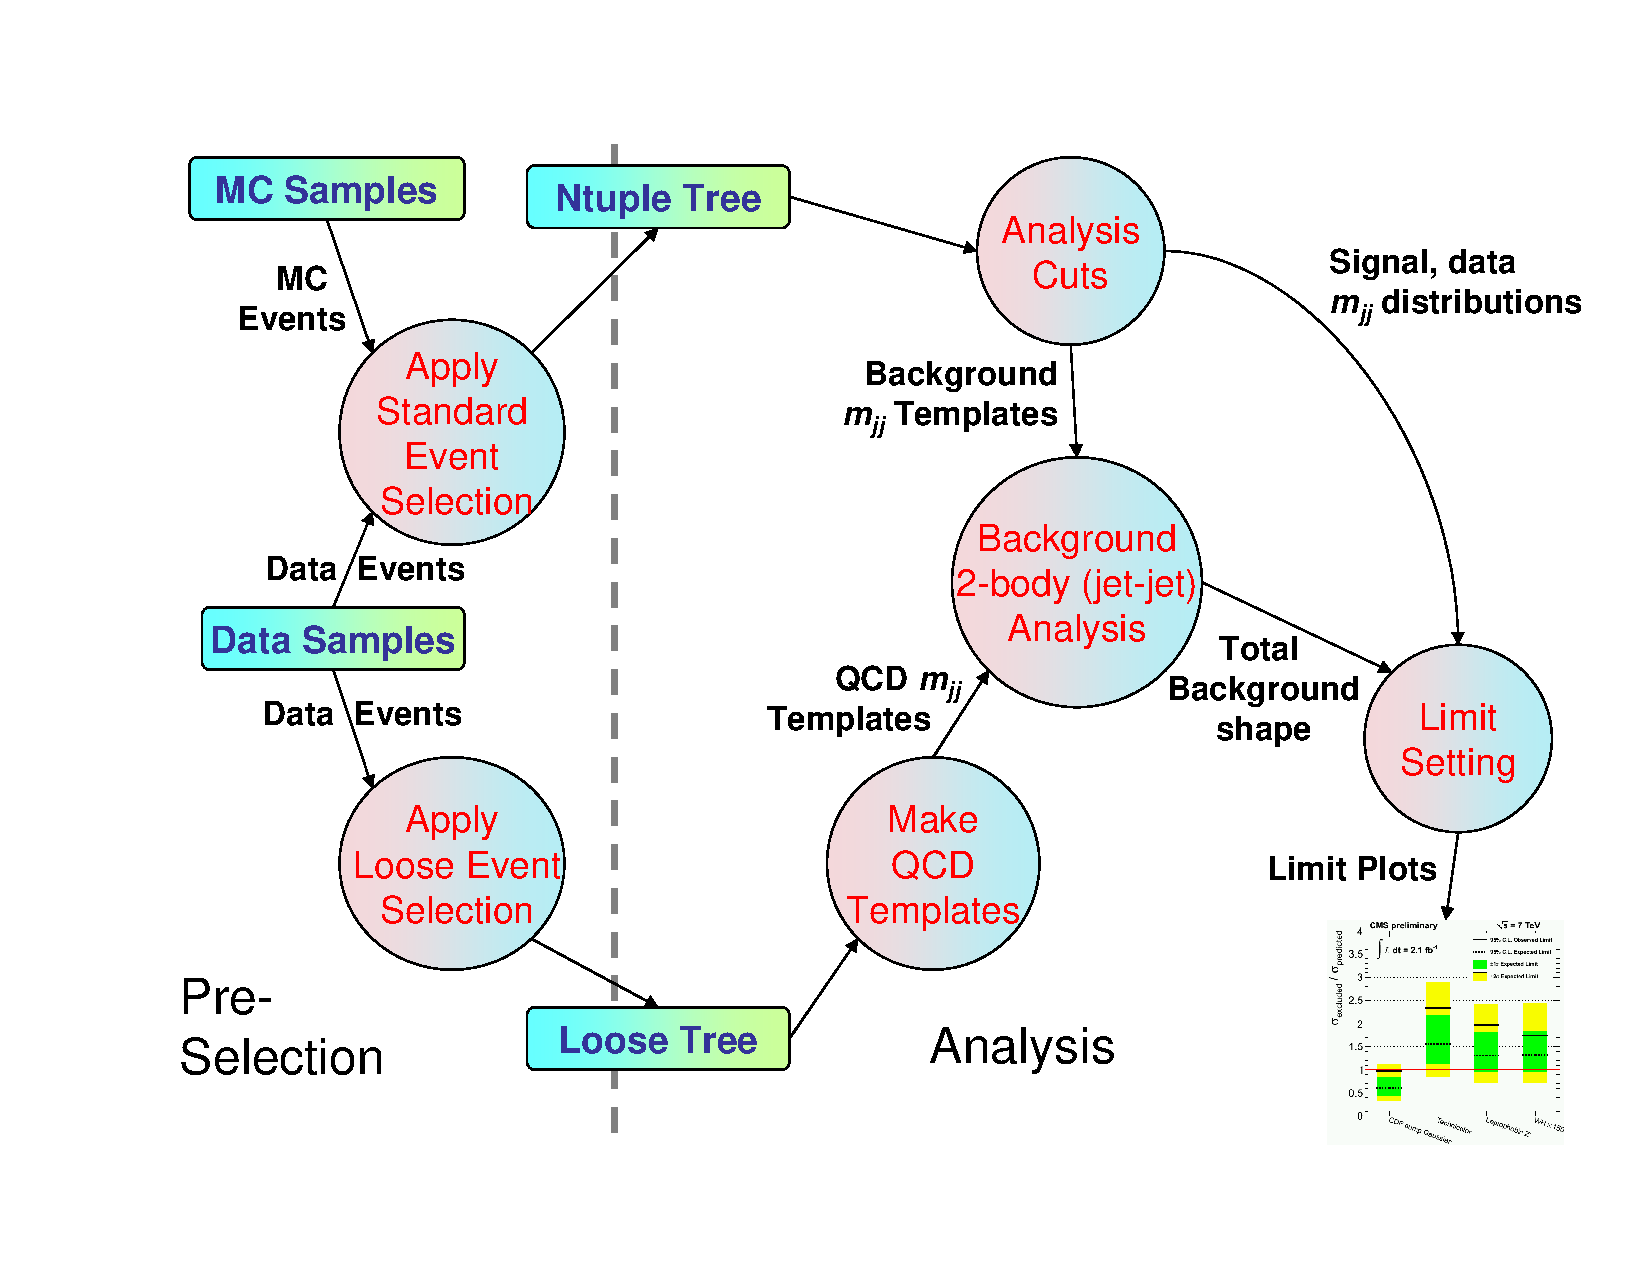
\includegraphics[width=\textwidth]{figs/mjjdfd0.pdf}
\caption{\label{fig:dfdlevel0}A schematic of the major elements of
the analysis in terms of data flows and transforms.}
\end{center}
\end{figure}
%%%%%%%%%%%%%%%%%%%
